\documentclass[../Main.tex]{subfiles}

\begin{document}

\section{Molecular Dynamics}

One of the most seminal works in Molecular Dynamics was Dr. Aneesur Rahman's 1964 paper \cite{Rahman1964} "Correlations in the Motion of Atoms in Lquid Argon", where a system of 864 argon atoms was simulated on a CDC 3600 computer using a predictor-corrector method and the computed quantities were matched against the empirical values. This was followed by a paper in 1967 \cite{Verlet1967} by Dr. Loup Verlet, which introduced the Verlet Integration method for the same model of 864 argon atoms.

In this section, we will look at replicating the aforementioned simulation for a system of 864 (a seemingly arbitrarily number) atoms of argon. Once set up, we will use the Velocity Verlet method (a modern variant of Verlet Integration) to calculate the motion of the particles, and observe how quantities such as temperature and local pressure behave over a long time period.

\subsection{Lennard-Jones Potential}

\begin{wrapfigure}{r}{0.5\textwidth}
\centering
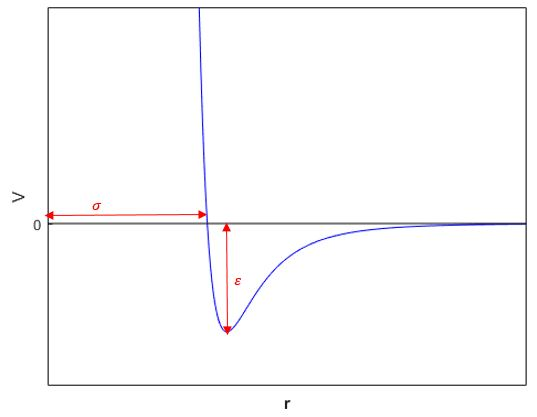
\includegraphics[scale=0.5]{lennard-jones_potential_graph}
\caption{Lennard-Jones Potential}
\label{fig:lennard-jones_potential}
\end{wrapfigure}

Before populating the argon atoms, we need to establish how the molecules will interact. We use the Lennard-Jones Potential to approximate the interaction with two atoms:
\begin{align}
	\vec{V}\left(\vec{r}_{ij}\right) = 4\varepsilon \left[ \left( \frac{\sigma}{r_{ij}}\right)^{12} - \left( \frac{\sigma}{r_{ij}}\right)^6 \right] \label{eqn:lennard-jones_potential}
\end{align}
where $\vec{r}_{ij}$ is the displacement between the i\textsuperscript{th} and the j\textsuperscript{th} atoms, $r_{ij} = \left\Vert\vec{r}_{ij}\right\Vert_{2}$, $\varepsilon$ is the potential well depth (a measure of strength of attraction of two atoms), and $\sigma$ is the distance at which the potential between two atoms is 0. The Lennard-Jones potential is a very simple model for the interactive forces between atoms; nevertheless it was found to suffice for modelling argon atoms in \cite{Rahman1964}. In fact, the simplicity of the Lennard-Jones potential contributes to speed of the simulation - given a system of $n$ atoms, the potential needs to be evaluated $\frac{n\left(n+1\right)}{2}$ times $\left(\mbox{as }r_{ij} = r_{ji}\right)$.

For an argon atom, $\varepsilon = 1.65 \times 10^{-21}$J and $\sigma = 3.40 \times 10^{-10}$m. However, the computer is prone to making errors when operating on such small numbers. In the next subsection, we will look at a technique that handles this problem.

\subsection{Forces}

We have that force $\vec{f}$ along the vector $\vec{r}_{ij}$ is given by:
\begin{align*}
\vec{f}\left(\vec{r}_{ij}\right) = -\frac{dV}{d\vec{r}_{ij}}
\end{align*}
Now,
\begin{align*}
\frac{dV}{dr_{ij}} = 4\varepsilon \left[ -12\left( \frac{\sigma}{r_{ij}}\right)^13 + 6\left( \frac{\sigma}{r_{ij}}\right)^7\right]
\end{align*}
and
\begin{align*}
\frac{dr_{ij}}{d\vec{r_{ij}}} = \frac{\vec{r}_{ij}}{r_{ij}}
\end{align*}
Hence, by the chain rule, we get that
\begin{align}
\vec{f}\left(\vec{r}_{ij}\right) & = -4\varepsilon \left[ -12\left( \frac{\sigma}{r_{ij}}\right)^13 + 6\left( \frac{\sigma}{r_{ij}}\right)^7\right] \times \frac{\vec{r}_{ij}}{r_{ij}} \nonumber \\
& = 48\varepsilon \left( \frac{\sigma}{r_{ij}}\right)^7 \left[ \left( \frac{\sigma}{r_{ij}}\right)^6 + \frac{1}{2}\left( \frac{\sigma}{r_{ij}}\right)\right] \times \frac{\vec{r}_{ij}}{r_{ij}} \label{eqn:lennard-jones_one_atom_force}
\end{align}

\subsection{Reduced Units}

As explained above, limits of a computer's precision can introduce floating point errors when expressing miniscule quantities such as potential in terms of the SI units. Hence, we scale - or "reduce" - these SI unis such that the quantities involved in the simulation have an order of magnitude of 1. This makes simplifies the calculations, and has the added benefit of making erroneous results easier to spot (as extreme values are now unlikely). We start off by expressing lengths in terms of $\sigma = 3.40 \times 10^{-10}$m, and energy in terms of $\varepsilon = 1.65 \times 10^{-21}$J. Then, the Lennard-Jones potential can be calculated as:
\begin{align}
	\vec{V}\left(\vec{r}_{ij}\right) = 4 \left[ \left( \frac{1}{r_{ij}}\right)^{12} - \left( \frac{1}{r_{ij}}\right)^6 \right] \label{eqn:lennard-jones_potential_reduced}
\end{align}
where $\vec{r}_{ij}$ and $r_{ij}$ have the same meaning as before, but are expressed as a multiple of $\sigma$.
Similarly, we reduce 
\end{document}